% Provided node and wireframe scaffolds; question versions contain no answer edges.
\newcommand{\ticketActor}[4]{%
 \coordinate (#1) at (#2,#3);
 \draw (#2,{#3+.62}) circle (.16);
 \draw (#2,{#3+.46})--(#2,{#3-.08});
 \draw ({#2-.3},{#3+.23})--({#2+.3},{#3+.23});
 \draw (#2,{#3-.08})--({#2-.27},{#3-.43});
 \draw (#2,{#3-.08})--({#2+.27},{#3-.43});
 \node[align=center,text width=2.25cm] at (#2,{#3-.77}) {#4};}
\newcommand{\ticketUseCaseNodes}{%
 \path[use as bounding box](0,.5)rectangle(16.8,-18.3);
 \draw(2.7,.1)rectangle(14.05,-18.1);
 \node[anchor=north,font=\bfseries]at(8.375,-.1){TokTickIT};
 \tikzset{ticketuc/.style={ellipse,draw,align=center,text width=2.7cm,minimum height=1.2cm,inner sep=3pt}}
 \node[ticketuc](create)at(6,-1.9){Create Ticket};
 \node[ticketuc](own)at(11,-1.9){View My Tickets};
 \node[ticketuc](queue)at(6,-4.7){View Ticket Queue};
 \node[ticketuc](update)at(11,-4.7){Update Ticket};
 \node[ticketuc](action)at(6,-7.5){Record Action};
 \node[ticketuc](notify)at(11,-7.5){Send Email};
 \node[ticketuc](attach)at(6,-10.3){Attach File};
 \node[ticketuc](validate)at(11,-10.3){Validate Attachment};
 \node[ticketuc](reassign)at(6,-13.1){Reassign Ticket};
 \node[ticketuc](resolve)at(11,-13.1){Resolve Ticket};
 \node[ticketuc](accounts)at(6,-15.9){Maintain Accounts};
 \node[ticketuc](gate)at(11,-15.9){Check Resolution Gate};
 \ticketActor{requester}{1.15}{-2.6}{Requester}
 \ticketActor{staff}{1.15}{-9.4}{IT Staff}
 \ticketActor{admin}{1.15}{-15.4}{Administrator}
 \node[draw,align=center,text width=2.1cm,minimum height=1.2cm](mail)at(15.55,-7.5){\textless\textless actor\textgreater\textgreater\\Email Gateway};}
\newcommand{\examTicketUseCase}{%
 \begin{center}\begin{tikzpicture}[x=1cm,y=1cm,font=\fontsize{9}{11}\selectfont]
 \ticketUseCaseNodes
 \end{tikzpicture}\end{center}}
\newcommand{\ticketStateNodes}{%
 \path[use as bounding box](0,.1)rectangle(16.8,-16.1);
 \tikzset{ticketstate/.style={draw,rounded corners=5pt,align=center,minimum width=3.9cm,minimum height=1.15cm,inner sep=4pt}}
 \node[circle,fill,inner sep=3pt](initial)at(7.6,-.35){};
 \node[ticketstate](new)at(3,-2.2){NEW};
 \node[ticketstate](open)at(3,-6){OPEN};
 \node[ticketstate](waiting)at(12.2,-2.2){WAITING\_FOR\_\\REQUESTER};
 \node[ticketstate](progress)at(12.2,-6){IN\_PROGRESS};
 \node[ticketstate](resolved)at(12.2,-9.8){RESOLVED};
 \node[ticketstate](cancelled)at(3,-13.6){CANCELLED};
 \node[ticketstate](closed)at(12.2,-13.6){CLOSED};
 \node[circle,draw,minimum size=4.5mm,inner sep=0pt](final)at(7.6,-15.7){};
 \fill(7.6,-15.7)circle(1.3mm);}
\newcommand{\examTicketState}{%
 \begin{center}\begin{tikzpicture}[x=1cm,y=.84cm,font=\fontsize{10}{12}\selectfont]
 \ticketStateNodes
 \end{tikzpicture}\end{center}}
\newcommand{\ticketNotationReference}{%
 \par\smallskip\noindent\begin{tikzpicture}[x=1cm,y=1cm,font=\fontsize{9}{11}\selectfont]
 \path[use as bounding box](0,.1)rectangle(16.8,-1.2);
 \node[anchor=west]at(0,-.25){*Required field};
 \draw(3.7,.05)rectangle(7.25,-.55);
 \node at(5.475,-.25){Editable};
 \fill[pattern=north east lines,pattern color=gray!40](8.1,.05)rectangle(11.65,-.55);
 \draw(8.1,.05)rectangle(11.65,-.55);
 \node[fill=white,inner sep=1pt]at(9.875,-.25){Read-only};
 \draw(12.5,.05)rectangle(16.7,-.55);
 \node at(14.6,-.25){LoV / Selection};
 \node[anchor=west]at(0,-1){Notation reference only; complete the blank frames below.};
 \end{tikzpicture}\par}
\newcommand{\examTicketQueue}{%
 \begin{center}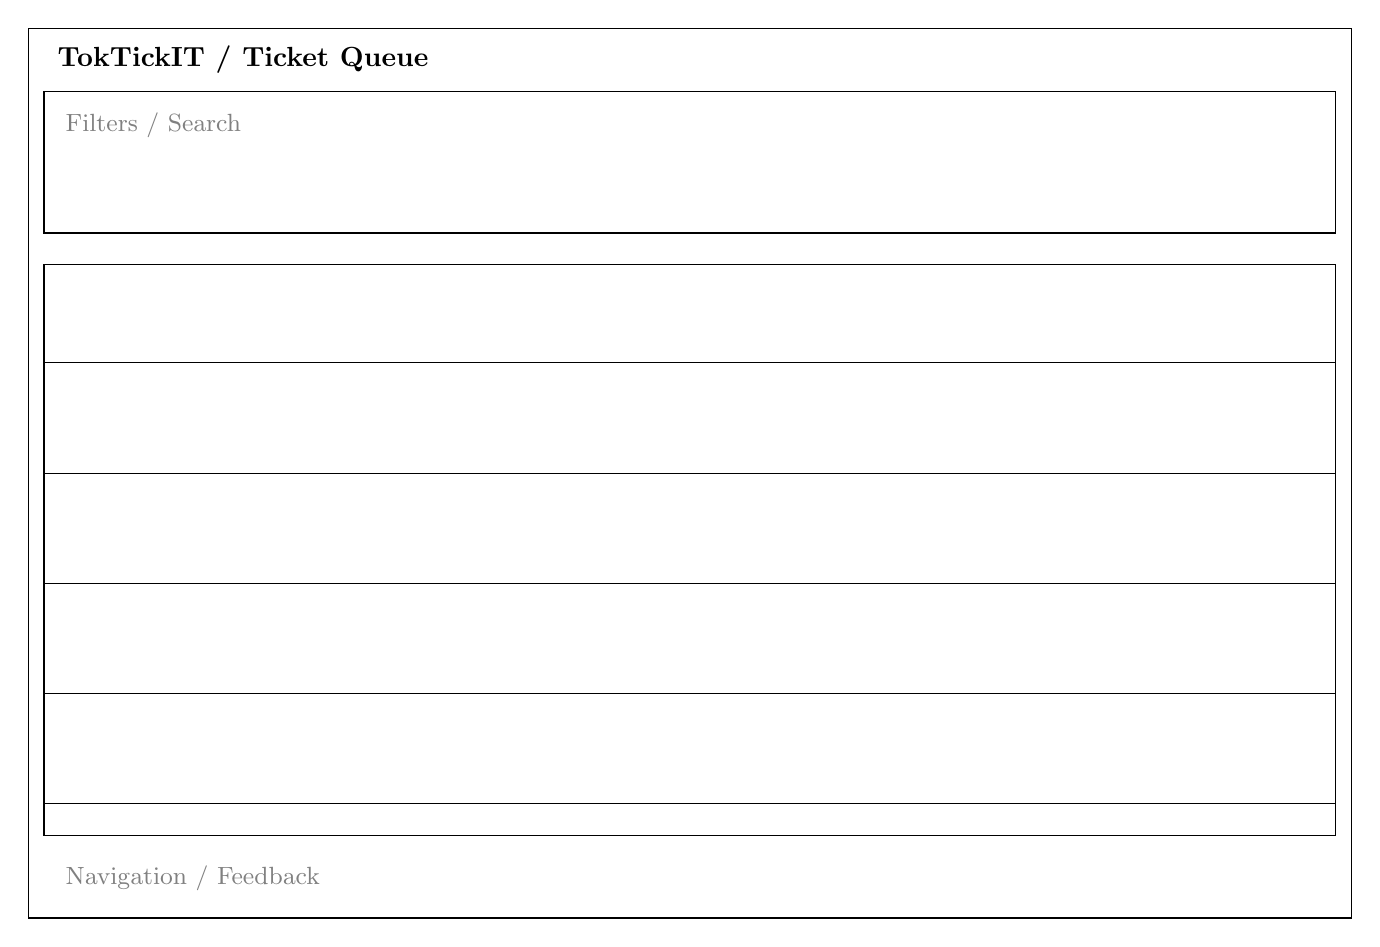
\begin{tikzpicture}[x=1cm,y=1cm,font=\fontsize{9}{11}\selectfont]
 \draw(0,0)rectangle(16.8,-11.3);
 \node[anchor=west,font=\bfseries]at(.25,-.4){TokTickIT / Ticket Queue};
 \draw(.2,-.8)rectangle(16.6,-2.6);
 \node[anchor=north west,text=gray]at(.35,-.95){Filters / Search};
 \draw(.2,-3)rectangle(16.6,-10.25);
 \foreach\y in{-4.25,-5.65,-7.05,-8.45}{\draw(.2,\y)--(16.6,\y);}
 \draw(.2,-9.85)--(16.6,-9.85);
 \node[anchor=west,text=gray]at(.35,-10.8){Navigation / Feedback};
 \end{tikzpicture}\end{center}}
\newcommand{\examTicketForm}{%
 \begin{center}\begin{tikzpicture}[x=1cm,y=1cm,font=\fontsize{9}{11}\selectfont]
 \draw(0,0)rectangle(16.8,-16.9);
 \node[anchor=west,font=\bfseries]at(.25,-.4){TokTickIT / Selected Ticket};
 \draw(.2,-.85)rectangle(16.6,-7.25);
 \node[anchor=north west,text=gray]at(.35,-1){Ticket information / Controls};
 \draw(.2,-7.65)rectangle(16.6,-12.7);
 \node[anchor=north west,text=gray]at(.35,-7.8){Actions / Threads};
 \draw(.2,-13.1)rectangle(16.6,-16.55);
 \node[anchor=north west,text=gray]at(.35,-13.25){Messages / Allowed actions};
 \end{tikzpicture}\end{center}}
